\documentclass[border=8pt]{standalone}
% Shared preamble for IronClaw thesis figures (standalone TikZ).
\renewcommand{\familydefault}{\sfdefault}
\usepackage{tikz}
\usetikzlibrary{arrows.meta,positioning,calc,fit,backgrounds,shapes.geometric,shapes.misc}

% IronClaw palette (matches slides.tex)
\definecolor{IronDark}{HTML}{1A2B3C}
\definecolor{IronBlue}{HTML}{2E86AB}
\definecolor{IronTeal}{HTML}{06A77D}
\definecolor{IronOrange}{HTML}{F18F01}
\definecolor{IronRed}{HTML}{C73E1D}
\definecolor{IronLight}{HTML}{F4F7F9}
\definecolor{IronGray}{HTML}{5D6D7E}

\tikzset{
  figtitle/.style={font=\large\bfseries\color{IronDark}, align=center},
  hostbox/.style={draw=IronBlue, rounded corners=5pt, fill=IronBlue!8,
                  line width=1pt, align=center, font=\small\color{white}},
  hostfill/.style={draw=IronBlue, rounded corners=4pt, fill=IronBlue,
                   line width=0.8pt, align=center, font=\small\color{white},
                   text width=3.1cm, minimum height=0.85cm},
  guestfill/.style={draw=IronOrange, rounded corners=4pt, fill=IronOrange!85,
                    line width=0.8pt, align=center, font=\small\color{white},
                    text width=3.1cm, minimum height=0.85cm},
  guestsoft/.style={draw=IronOrange, rounded corners=4pt, fill=IronOrange!25,
                    line width=0.8pt, align=center, font=\small\color{IronDark},
                    text width=3.1cm, minimum height=0.75cm},
  arrow/.style={-{Latex[length=2.6mm,width=2mm]}, line width=0.9pt, IronDark},
  biarrow/.style={{Latex[length=2.6mm,width=2mm]}-{Latex[length=2.6mm,width=2mm]},
                  line width=0.9pt, IronDark},
  note/.style={font=\footnotesize\color{IronGray}, align=center},
}

\begin{document}
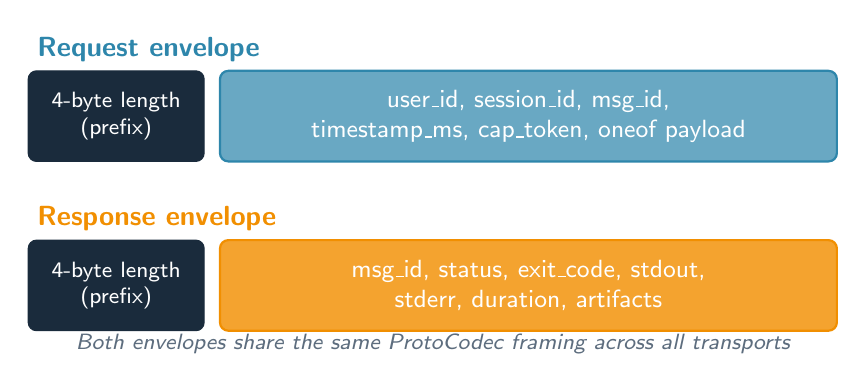
\begin{tikzpicture}
  \tikzset{
    lenpre/.style={draw=IronDark, fill=IronDark, text=white, rounded corners=3pt,
                   minimum height=1.15cm, text width=2.0cm, align=center, font=\footnotesize},
    payload/.style={rounded corners=3pt, minimum height=1.15cm, text width=7.6cm,
                    align=center, font=\small, text=white, line width=0.8pt},
  }

  % Request envelope
  \node[font=\normalsize\bfseries\color{IronBlue}, anchor=west] at (0,3.4) {Request envelope};
  \node[lenpre, anchor=west] (rpre) at (0,2.55) {4-byte length\\(prefix)};
  \node[payload, draw=IronBlue, fill=IronBlue!72, anchor=west] (rpay)
        at ($(rpre.east)+(0.18,0)$)
        {user\_id, session\_id, msg\_id,\\timestamp\_ms, cap\_token, oneof payload};

  % Response envelope
  \node[font=\normalsize\bfseries\color{IronOrange}, anchor=west] at (0,1.25) {Response envelope};
  \node[lenpre, anchor=west] (ppre) at (0,0.4) {4-byte length\\(prefix)};
  \node[payload, draw=IronOrange, fill=IronOrange!82, anchor=west] (ppay)
        at ($(ppre.east)+(0.18,0)$)
        {msg\_id, status, exit\_code, stdout,\\stderr, duration, artifacts};

  \node[note, anchor=north] at ($(ppre.west)!0.5!(ppay.east)+(0,-0.5)$)
        {\itshape Both envelopes share the same ProtoCodec framing across all transports};

\end{tikzpicture}
\end{document}
